% Beamer Presentation
% Nicholas R. Jenkins (nicholas.jenkins@email.ucr.edu)
% Department of Political Science
% University of California, Riverside
%
% Presentation for: Article_Title
% ---------------------------------------------------------------------------

% Document and Theme Setup %
\documentclass[12pt, aspectratio=169]{beamer}
\usetheme{default}
\usecolortheme{crane}
\useoutertheme[subsection=false, footline=authortitle]{miniframes} 
\usefonttheme{default}  	% default, professionalfonts, serif, structurebold, structureitalicserif, structuresmallcapsserif,
\setbeamercovered{transparent} 
\setbeamertemplate{navigation symbols}{}

% Remove Navigation Dots at the top of the slides %
\makeatletter
\def\beamer@writeslidentry{\clearpage\beamer@notesactions}
\makeatother

% Load Packages %
\usepackage[utf8]{inputenc}
\usepackage[english]{babel}
\usepackage{csquotes}
\usepackage{amsmath}
\usepackage{amsfonts}
\usepackage{amssymb}
\usepackage{graphicx}
\usepackage{bookmark}
\usepackage{appendixnumberbeamer}
\usepackage{tikz}
\usetikzlibrary{positioning}
\usepackage{tabu}
\usepackage{graphicx}
\usepackage{longtable}
\usepackage{booktabs}
\usepackage{amsfonts}
\usepackage{pdflscape}
\usepackage{footmisc}
\usepackage{subfig}
\usepackage{bm}
\usepackage{longtable}
\usetikzlibrary{shapes, shadows, arrows}
\usepackage{rotating}
\usepackage{multirow}
\usepackage[section]{placeins}
\usepackage{pgfplots}


% Define Colors %
% These are the UC Riverside colors found here: http://creativedesign.ucr.edu/ism/colors.html
\definecolor{UCRGray}{RGB}{122, 110, 103}
%\definecolor{UCGold}{RGB}{255, 181, 17} % UC System Color
%\definecolor{UCBlue}{RGB}{18, 149, 216} % UC System Color
\definecolor{UCGold}{RGB}{241, 171, 0} % UC Riverside Official Color
\definecolor{UCBlue}{RGB}{45, 108, 192} % UC Riverside Official Color
\definecolor{UCBlack}{RGB}{0, 0, 0} 
\definecolor{lightgray}{RGB}{215, 215, 215}


% Set Colors %
\setbeamercolor*{palette tertiary}{fg=black, bg=UCGold} % Section color (color of navigation header and dots)
\setbeamercolor{frametitle}{fg=UCBlue, bg=white} % Color of the title bar on each frame
\setbeamercolor{title}{fg=UCBlue, bg=lightgray} 
\setbeamercolor{alerted text}{fg=UCGold} % Color of alert text and block
\setbeamercolor{example text}{fg=UCBlue} % Color of example text
\setbeamercolor{enumerate item}{fg=UCBlue} % Number color
\setbeamercolor{itemize item}{fg=UCBlue} % Bullet point color
\setbeamertemplate{itemize items}[square] % Bullet point style 
\setbeamercolor{button}{bg=lightgray,fg=UCBlue} % Button Color



% University Macros %
\newcommand{\ucr}{Department of Political Science \\ 
University of California, Riverside \\
\textit{nicholas.jenkins@email.ucr.edu}}


% Bibliography Setup %
\usepackage[authordate, natbib, isbn=false, url=false, doi=false, backend=biber]{biblatex-chicago} 
\bibliography{/Users/nick/Documents/Research/References/BibTeX/biblatex.bib}


% Title Page Information %
\title[Rejecting PACs and Contribution Patterns]{Transparency or Deception? How Rejecting PAC Contributions Affects Contribution Patterns}
%\subtitle{Subtitle}

% Single Author
\author{Nicholas R. Jenkins}
\institute{\ucr}

% Multiple Authors
%\author[Nick]{Nicholas R. Jenkins \inst{1} \and author2 \inst{2}} 
%\institute[shortinst]{\inst{1} \ucr \and \inst{2} affiliation for author2}

\date{\today}


%\subject{} 

% Title Page and Graphics %
\pgfdeclareimage[height=2cm]{university-logo}{UCR-3.png} % Choose UCR-1, UCR-2, UCR-3, or UCR-4 for a logo on each slide
\titlegraphic{\hfill\includegraphics[height=2cm]{UCR-3}} % Title Page Logo
%\logo{\pgfuseimage{university-logo}} % Logo on Each Slide


% Begin Presentation %
\begin{document}


% Title Page
\begin{frame}
\titlepage
\end{frame}


\section{Motivation} \label{sec: motivation}

\begin{frame}{Motivation}
		\begin{tikzpicture}
		\node (1) at (4,12) {\includegraphics[width=0.7\linewidth]{5}}; 
		\node (3) at (2,6) [yshift=2cm] {\includegraphics[width=0.6\linewidth]{3}}; 
	\end{tikzpicture}
\end{frame}


\section{Motivation} \label{sec: motivation}

\begin{frame}{Motivation}
		\begin{tikzpicture}
		\node (2) at (-1,8.3) [yshift=2cm] {\includegraphics[width=0.6\linewidth]{2}};
		\node (2) at (0,4) [yshift=2cm] {\includegraphics[width=0.6\linewidth]{1}};
		\node (2) at (4,6) [yshift=2cm] {\includegraphics[width=0.6\linewidth]{4}};
	\end{tikzpicture}
\end{frame}

% Table of Contents Slide
%\begin{frame}
%\tableofcontents
%\end{frame}


\section{Perceptions of Money in Politics} \label{sec: framework}


\begin{frame}{Motivating individuals?}

	\begin{alertblock}{Hypothesis 1}
Candidates that pledge to reject corporate PAC contributions will receive an increase in individual small-dollar donations.
\end{alertblock} \pause

	\begin{itemize}
		\item People generally hold negative views of money in politics {\tiny \citep{lubenow2001}} \pause
		\item Funding sources might affect voter perceptions of candidates {\tiny \citep{bowler2016}} \pause
		\item Pledging to reject corporate PAC money might signal trustworthiness \pause
		\item Discussions of these pledges and requests for small-dollar donations go hand-in-hand
	\end{itemize}
	
\end{frame}


\begin{frame}{Parties with their fingers crossed?}

\begin{alertblock}{Hypothesis 2}
Candidates that reject corporate PAC money will receive more contributions from partisan sources.
\end{alertblock} \pause

\begin{itemize}
	\item Why not reject all PAC money? \pause
	\item Taking the pledge is also risky \pause
	\item Will political parties just hope that their candidates raise enough money? \pause
	\begin{itemize}
		\item Parties give strategically! {\tiny \citep{wilcox1989, currinder2003, herrnson2009}}
	\end{itemize}
\end{itemize}

\end{frame}


\begin{frame}{Corporations just give up?}

\begin{alertblock}{Hypothesis 3}
Candidates that reject corporate PAC money will receive more contributions from individuals associated with business and ideological interests.
\end{alertblock} \pause

\begin{itemize}
	\item Opportunity cost of not making contributions is very high! {\tiny \citep{grier1991}} \pause
	\item Corporations can ``bundle" individual donations to candidates 
\end{itemize}

\end{frame}


\begin{frame}{The Trade-off Summarized}
	\begin{figure}[!htb]
\centering
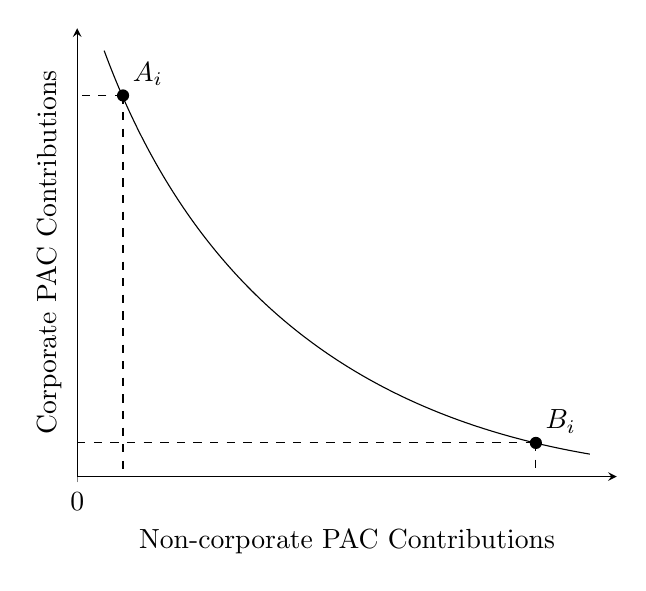
\begin{tikzpicture}
\begin{axis}[
    axis x line=bottom,
    axis y line=left,
    xmin=0, xmax=10, 
    ymin=0, ymax=10,
    xlabel={Non-corporate PAC Contributions},
    ylabel={Corporate PAC Contributions},
    ytick=\empty,
    xtick={0},
    extra y tick style={align=center, font=\scriptsize},
    ]
    \draw (axis cs:0.5,9.5) to [bend right=30] coordinate[pos=0.2] (l_i) (axis cs:9.5,0.5);
    \fill (axis cs:0.85,8.5) circle (2.2pt) node[above right] {$A_i$};

    \fill (axis cs:8.5,0.75) circle (2.2pt) node[above right] {$B_i$};
    
    \draw[dashed, thin] (axis cs:0.85,8.5) -- (axis cs:0.85,0);
    \draw[dashed, thin] (axis cs:0.85,8.5) -- (axis cs:0,8.5);
    \draw[dashed, thin] (axis cs:8.5,0.75) -- (axis cs:8.5,0);
    \draw[dashed, thin] (axis cs:0,0.75) -- (axis cs:8.5,0.75); 
\end{axis}
\end{tikzpicture}
\label{fig: iso map}
\end{figure}
\end{frame}


\section{Methods} \label{sec: methods}

\begin{frame}{Sample Information}
	\begin{itemize}
		\item Sample of candidates in the 2018 Congressional midterm election \pause
		\item Only Democrats who won their election (167)
	\end{itemize}
\end{frame}

\begin{frame}{Exploratory Data Analysis}

\begin{figure}[!htb]
    \centering
    \includegraphics[width=0.65\linewidth]{all_candy.pdf}

\end{figure}

\end{frame}


\begin{frame}{Exploratory Data Analysis}

\begin{figure}[ht]
    \centering
    \includegraphics[width=1\linewidth]{spending_candy.pdf}
\end{figure}

\end{frame}


\begin{frame}{Model Definition}

\begin{itemize}
	\item Campaign contributions follow a gamma distribution ($y \in  \mathbb{R}^+$)
\end{itemize}

\begin{figure}[!htb]
    \centering
    \includegraphics[width=0.5\linewidth]{gamma.pdf}
\end{figure}

\end{frame}


\begin{frame}{Model Definition}

\begin{itemize}
	\item But, zeros are also possible!
\end{itemize}

\begin{figure} \pause 
    \centering
    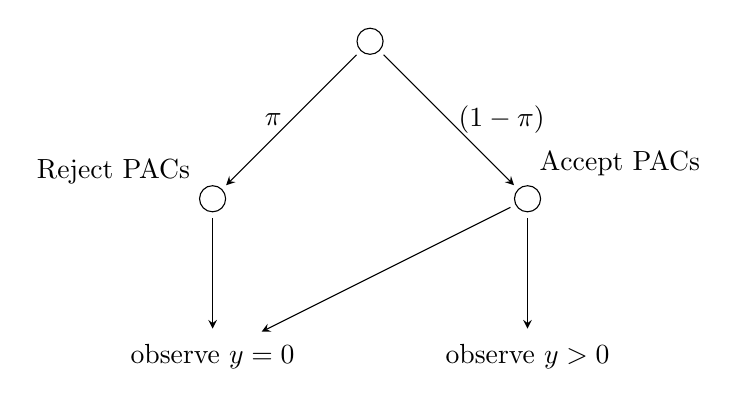
\begin{tikzpicture}[
        node distance=2.0cm,
      scale=0.5,
      level/.style={thick},
      virtual/.style={thick,densely dashed},
      trans/.style={->,shorten >=2pt,shorten <=2pt,>=stealth},
      classical/.style={thin,double,<->,shorten >=4pt,shorten <=4pt,>=stealth}
    ]
    \node(a)[circle, draw=black, label={160:Reject PACs}] {};
    \node(z)[right of=a] {};
    \node(b)[circle, draw=black, right of=z, label={80:Accept PACs}] {};
    \node(c)[circle, draw=black, above of=z] {};
    \node(d)[below of=a] {observe $y = 0$};
    \node(e)[below of=b] {observe $y > 0$};
    
    \draw [trans] (c) -- (a) node[midway, left] {$\pi$};
    \draw [trans] (c) -- (b) node[midway, right] {$(1 - \pi)$};
    \draw [trans] (a) -- (d);
    \draw [trans] (b) -- (e);
    \draw [trans] (b) -- (d);
    \end{tikzpicture}
\end{figure}

\end{frame}


\begin{frame}{Percentage of Zeros}

\begin{figure}[!htb]
    \centering
    \includegraphics[width=0.77\linewidth]{zero_candy.pdf}
\end{figure}

\end{frame}


\begin{frame}{Model Definition}

\begin{align}
f(y) = \left\{ \begin{array}{cc} 
                \pi & \hspace{5mm} \text{if $y = 0$} \\
                (1 - \pi) \text{Gamma}(k, \theta) & \hspace{5mm}  \text{if $y > 0$} \\
                \end{array} \right.
\end{align}

\end{frame}


\begin{frame}{Model Definition}

\begin{align}
    y_i &\sim \text{ZGamma}(\pi_i, \mu_i, \theta_i) \\
    \log \frac{\pi_i}{1 - \pi_i} &= \alpha_{\pi} + \beta_{1\pi} (\text{No PACs})_i + \beta_{2\pi} (\text{New Member})_i \\
   \log( \mu_i) &= \alpha_{\mu} + \beta_{1\mu} (\text{No PACs})_i + \bm{X} \bm{\beta_{\mu}}
\end{align} \pause

\begin{itemize}
	\item Yes, priors are subjective ... but so are likelihood and link functions!
\end{itemize}

\end{frame}


\section{Findings} \label{sec: findings}

\begin{frame}{Are the pledges effective?} \label{pac results}

\begin{figure}
  \centering
  \subfloat[The Effect of Rejecting Corporate PAC Contributions on the Amount of PAC Contributions\label{fig:a}]{\includegraphics[width=0.47\linewidth]{pac_coef.pdf}}\qquad
  \subfloat[The Effect of Rejecting Corporate PAC Contributions on the Probability of Receiving PAC Contributions\label{fig:b}]{\includegraphics[width=0.47\linewidth]{pac_probs.pdf}}
\end{figure}

\hyperlink{pac priors}{\beamerbutton{Prior Simulations}}

\end{frame}


\begin{frame}{Are the pledges effective?}

\begin{figure}[!htb]
    \centering
    \includegraphics[width=1\linewidth]{pac_preds.pdf}
    \label{fig: pac preds}
\end{figure}

\end{frame}


\begin{frame}{Parties with their fingers crossed?} \label{party results}

\begin{figure}
  \centering
  \subfloat[The Effect of Rejecting Corporate PAC Contributions on the Amount of Contributions from Party Organizations\label{fig:a}]{\includegraphics[width=0.47\linewidth]{party_coef.pdf}}\qquad
  \subfloat[The Effect of Rejecting Corporate PAC Contributions on the Probability of Receiving Party Contributions\label{fig:b}]{\includegraphics[width=0.47\linewidth]{prty_probs.pdf}}
\end{figure}

\hyperlink{party priors}{\beamerbutton{Prior Simulations}}

\end{frame}


\begin{frame}{Parties with their fingers crossed?}

\begin{figure}[!htb]
    \centering
    \includegraphics[width=1\linewidth]{party_preds.pdf}
    \label{fig: pac preds}
\end{figure}

\end{frame}


\begin{frame}{Corporations just give up?} \label{indiv results}

\begin{figure}
  \centering
  \subfloat[The Effect of Rejecting Corporate PAC Contributions on the Amount of Contributions from Individuals\label{fig:a}]{\includegraphics[width=0.47\linewidth]{indv_coef.pdf}}\qquad
  \subfloat[The Effect of Rejecting Corporate PAC Contributions on the Probability of Receiving Individual Contributions.\label{fig:b}]{\includegraphics[width=0.47\linewidth]{indiv_probs.pdf}}
\end{figure}

\hyperlink{indiv priors}{\beamerbutton{Prior Simulations}}

\end{frame}


\begin{frame}{Corporations just give up?}

\begin{figure}[!htb]
    \centering
    \includegraphics[width=1\linewidth]{indv_preds.pdf}
    \label{fig: pac preds}
\end{figure}

\end{frame}


\section{Summary} \label{sec: summary}

\begin{frame}{Summary}
\begin{itemize}
	\item Pledging to reject corporate PAC contributions is associated with: \pause
	\begin{itemize}
		\item $\downarrow$ contributions from ideological, labor, and business PACs \pause
		\item $\uparrow$ contributions from political PACs and individuals \pause
		\item $\uparrow$ in small and large dollar contributions \pause
		\item $\uparrow$ in contributions from individuals affiliated with ideological and business interests
	\end{itemize}
\end{itemize}
\end{frame}

% Appendixes
\begin{appendix}
	
\begin{frame}{Priors for PAC Models} \label{pac priors}

\begin{figure}
  \centering
  \subfloat[Priors for Model Intercepts\label{fig:a}]{\includegraphics[width=0.46\linewidth]{pac_int.pdf}}\qquad
  \subfloat[Priors for Model Slopes\label{fig:b}]{\includegraphics[width=0.46\linewidth]{pac_slopes.pdf}}
\end{figure}
		
		\hyperlink{pac results}{\beamerbutton{PAC Results}}
		
\end{frame}

\begin{frame}{Priors for Political PAC Models} \label{party priors}

\begin{figure}
  \centering
  \subfloat[Priors for Model Intercepts\label{fig:a}]{\includegraphics[width=0.46\linewidth]{party_int.pdf}}\qquad
  \subfloat[Priors for Model Slopes\label{fig:b}]{\includegraphics[width=0.46\linewidth]{party_slopes.pdf}}
\end{figure}

\hyperlink{party results}{\beamerbutton{Party Results}}
		
\end{frame}

\begin{frame}{Priors for Individual Models} \label{indiv priors}

\begin{figure}
  \centering
  \subfloat[Priors for Model Intercepts\label{fig:a}]{\includegraphics[width=0.46\linewidth]{indiv_int.pdf}}\qquad
  \subfloat[Priors for Model Slopes\label{fig:b}]{\includegraphics[width=0.46\linewidth]{indiv_slopes.pdf}}
\end{figure}

\hyperlink{indiv results}{\beamerbutton{Individual Results}}
		
\end{frame}
	
\end{appendix}




\end{document}